% ---------------------------------------------------------------------------
% MATS research poster - LaTeX/beamer port of the MATS Google Slides template
%
% Page size: 24in x 36in portrait (same as the Slides template).
% Compile:   latexmk -pdf poster.tex
%
% Poster for P1: Can Power Draw Constrain Covert Compute? (power-to-flops),
% with a closing nod to the companion project
% (detecting-training-from-power-traces). The earlier two-project umbrella
% version is preserved as poster_umbrella.tex.bak.
% Figures live in ./figures/ (copied from the repo; exchange_scales.pdf is
% built standalone from the paper's TikZ, see figures/exchange_scales.tex).
% ---------------------------------------------------------------------------
\documentclass[final]{beamer}
\usepackage[size=custom,width=60.96,height=91.44,scale=1.0]{beamerposter}

\usepackage[T1]{fontenc}
\usepackage{libertine}          % Linux Libertine (serif) + Biolinum (sans)
\usepackage{tikz}
\graphicspath{{figures/}}

% --- colours (sampled from the Slides template; tweak here) ----------------
\definecolor{matsmaroon}{HTML}{8A1B2E}   % sidebar / accent red
\definecolor{sidebarmuted}{HTML}{C9909C} % small-caps labels in the sidebar
\definecolor{maintext}{HTML}{1A1A1A}
\definecolor{bodygray}{HTML}{333333}
\definecolor{subtitlegray}{HTML}{595959}
\definecolor{captiongray}{HTML}{6E6E6E}
\definecolor{phbg}{HTML}{F4F2EC}         % figure-placeholder background
\definecolor{phborder}{HTML}{B8B8B8}

% --- geometry ---------------------------------------------------------------
\newlength{\sidebarwidth}\setlength{\sidebarwidth}{0.325\paperwidth}
\newlength{\sidebarpad}\setlength{\sidebarpad}{2.4cm}
\newlength{\mainpad}\setlength{\mainpad}{2.8cm}

\setbeamertemplate{navigation symbols}{}
\setbeamertemplate{headline}{}
\setbeamertemplate{footline}{}
\setbeamersize{text margin left=0pt, text margin right=0pt}
\setbeamercolor{normal text}{fg=bodygray, bg=white}

% maroon sidebar painted as the frame background
\setbeamertemplate{background}{%
  \begin{tikzpicture}
    \useasboundingbox (0,0) rectangle (\paperwidth,\paperheight);
    \fill[matsmaroon] (0,0) rectangle (\sidebarwidth,\paperheight);
  \end{tikzpicture}}

% --- font sizes (absolute, independent of beamerposter scaling) ------------
\newcommand{\titlefont}{\rmfamily\bfseries\fontsize{66}{78}\selectfont}
\newcommand{\subtitlefont}{\sffamily\fontsize{27}{35}\selectfont}
\newcommand{\sectionfont}{\rmfamily\bfseries\fontsize{36}{42}\selectfont}
\newcommand{\bodyfont}{\sffamily\fontsize{21}{27}\selectfont}
\newcommand{\sidebodyfont}{\sffamily\fontsize{23}{30}\selectfont}
\newcommand{\sidelabelfont}{\rmfamily\fontsize{26}{32}\selectfont}
\newcommand{\tldrfont}{\rmfamily\fontsize{28}{38}\selectfont}
\newcommand{\captionfont}{\sffamily\fontsize{19}{25}\selectfont}
\newcommand{\finefont}{\sffamily\fontsize{18}{24}\selectfont}
\newcommand{\logofont}{\rmfamily\fontsize{90}{90}\selectfont}

% --- building blocks --------------------------------------------------------
% small-caps muted label in the sidebar, e.g. \sidebarlabel{Authors}
\newcommand{\sidebarlabel}[1]{%
  {\color{sidebarmuted}\sidelabelfont\scshape\MakeLowercase{#1}\par}%
  \vspace{0.5cm}}

% thin white separator rule in the sidebar
\newcommand{\sidebarrule}{%
  \vspace{0.8cm}{\color{white}\rule{\linewidth}{1.2pt}\par}\vspace{0.8cm}}

% numbered contribution item, e.g. \contribution{1}{First contribution.}
\newcommand{\contribution}[2]{%
  \makebox[1.6em][l]{\bfseries #1.}%
  \parbox[t]{\dimexpr\linewidth-1.6em\relax}{\raggedright #2}\par
  \vspace{0.6cm}}

% main-column section heading with maroon underline
\newcommand{\postersection}[1]{%
  \vspace{0.35cm}%
  {\color{matsmaroon}\sectionfont #1\par}%
  \vspace{0.12cm}%
  {\color{matsmaroon}\rule{\linewidth}{2pt}\par}%
  \vspace{0.35cm}}

% maroon bullet item for the main column
\newcommand{\bulletitem}[1]{%
  \par\hangindent=1.2em\hangafter=1
  \makebox[1.2em][l]{\color{matsmaroon}\textbullet}#1\par\vspace{0.2cm}}

% inline red-bullet separator for run-in lists, e.g. A\redsep B\redsep C
\newcommand{\redsep}{\;{\color{matsmaroon}\textbullet}\;}

% figure caption, e.g. \postercaption{Figure 1. Description of the figure.}
\newcommand{\postercaption}[1]{%
  \vspace{0.25cm}{\color{captiongray}\captionfont #1\par}}

% QR code image with a small label underneath
\newcommand{\posterqr}[2]{% #1 = image file, #2 = label
  \begin{minipage}[t]{6.5cm}
    \centering
    \includegraphics[width=6cm]{#1}\\[0.35cm]
    {\finefont\color{white}#2}
  \end{minipage}}

% ===========================================================================
\begin{document}
\begin{frame}[t]
\vspace{0.9cm}
\begin{columns}[T]

% ===================== SIDEBAR =============================================
\begin{column}{\sidebarwidth}
\centering
\begin{minipage}[t][0.93\paperheight][t]{\dimexpr\sidebarwidth-2\sidebarpad\relax}
\color{white}\sidebodyfont\raggedright

% --- SIDEBAR: LOGO ---------------------------------------------------------
\noindent
\includegraphics[width=0.75\linewidth]{mats_white}\par
\vspace{2cm}

% --- SIDEBAR: AUTHORS --------------------------------------------------------
\sidebarlabel{Authors}
Tom Kimpson\textsuperscript{1,2}\\[0.25cm]
Mauricio Baker\textsuperscript{3}\\[0.25cm]
Emlyn Graham\textsuperscript{2}\\[0.25cm]
Anjay Friedman\textsuperscript{3}\\[0.25cm]
Maximus Rafla\textsuperscript{3}\\[0.25cm]
Coby Joseph\textsuperscript{3}\\[0.7cm]
{\finefont
\textsuperscript{1}University of Melbourne\\[0.15cm]
\textsuperscript{2}MATS\quad
\textsuperscript{3}RAND Corporation\par}

\sidebarrule

% --- SIDEBAR: TLDR -----------------------------------------------------------
\sidebarlabel{TL;DR}
{\tldrfont How much compute can an operator hide from a power meter? We
derive the answer in closed form and measure it on real GPUs: 0.4
machines' worth, falling to 0.07 under reasonable assumptions.\par}

\sidebarrule

% --- SIDEBAR: CONTRIBUTIONS --------------------------------------------------
\sidebarlabel{Contributions}
\contribution{1}{A closed-form floor $\beta$: the largest covert
computation a power trace cannot rule out, in machines of declared
capacity.}
\contribution{2}{Every input of the closed form measured on NVIDIA A100s
--- band edges, overhead, and the marginal cost of covert work.}
\contribution{3}{Explicit cheating strategies that hide 0.41 machines of
covert compute behind a trace the meter accepts.}
\contribution{4}{A ladder of verifier capabilities and assumptions that
shrink the floor --- requiring covert work to be \emph{useful} pushes
$\beta$ down to $0.07$.}

\vspace{0.5cm}

% --- SIDEBAR: READ MORE ------------------------------------------------------
\sidebarlabel{Read more}
{\finefont
Paper \& code: github.com/tomkimpson/power-to-flops\\[0.2cm]
Companion: github.com/tomkimpson/\\
\hspace*{1em}detecting-training-from-power-traces\\[0.2cm]
Contact: tom.kimpson@unimelb.edu.au\par}

\vfill

% --- SIDEBAR: QR CODE --------------------------------------------------------
\posterqr{qr}{Read more}

\end{minipage}
\end{column}

% ===================== MAIN COLUMN =========================================
\begin{column}{\dimexpr\paperwidth-\sidebarwidth\relax}
\centering
\begin{minipage}[t][0.93\paperheight][t]{\dimexpr\paperwidth-\sidebarwidth-2\mainpad\relax}
\bodyfont\color{bodygray}\raggedright

% --- TITLE BLOCK -------------------------------------------------------------
{\color{maintext}\titlefont Can Power Draw Constrain Covert Compute?\par}
\vspace{0.3cm}
%{\color{subtitlegray}\subtitlefont How tightly can an off-chip power meter
%bound total operations, against an operator who cheats?\par}
%\vspace{0.9cm}
%{\color{matsmaroon}\rule{\linewidth}{2pt}\par}

% --- MOTIVATION --------------------------------------------------------------
\postersection{Motivation}
\bulletitem{International agreements on frontier AI require \textit{verification}: an outside party must be
able to check what an operator actually ran, against an operator who may
cheat and try to hide their computation.}
\bulletitem{Hardware mechanisms for verification typically rely on reading silicon
the operator controls.}
\bulletitem{Off-chip analogue sensors (e.g. a power meter) have been identified as a
potential verification channel that is beyond the operator's reach.}
\bulletitem{We ask the question: given only the power trace,
\textbf{how much computation can the operator hide?}}

% --- PHYSICS -------------------------------------------------------------------
\postersection{From power to FLOPs?}
\bulletitem{A power meter sees only $P(t) = r(t)\,F(t) + P_0(t)$: an operation rate
$F$ priced at an exchange rate $r$ [J/op], on top of an overhead draw
$P_0$.}
\bulletitem{The rate $r$ is not a device constant --- it varies with how the
machine is run.}
\bulletitem{Given $P(t)$ (or its integral $E = \int P(t) dt$) we want to know $F(t)$ (or its integral $C=\int F dt$); an inverse problem.}
\bulletitem{\textbf{BUT} the equation is non-injective and so cannot be inverted.}
\bulletitem{We instead bound the width of the covert compute interval, $\beta \propto C_{\rm high} - C_{\rm low}$}

\vspace{0.25cm}
\begin{center}
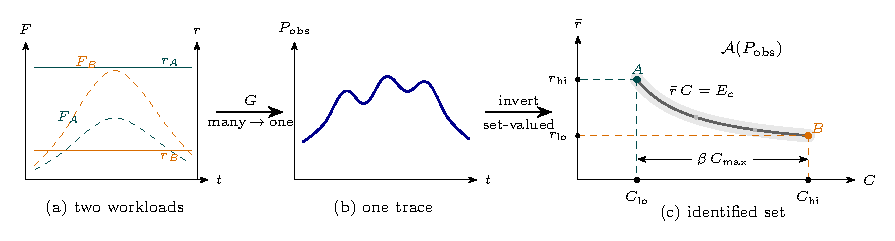
\includegraphics[width=0.73\linewidth]{noninjective}
\end{center}
\postercaption{Figure 1. Two workloads whose products $rF$ coincide drive
one trace; inverting recovers only the interval
$[C_{\mathrm{lo}}, C_{\mathrm{hi}}]$, whose width relative to capacity is
the floor $\beta$.}

\vspace{0.35cm}
\noindent
\begin{minipage}[c]{0.35\linewidth}
\bulletitem{The dynamic power law factorises
$r = \alpha\,\kappa\,C_{\mathrm{eff}}\,V^2$ --- operands, format,
locality, voltage: all chosen by the prover.}
\bulletitem{The overhead $P_0$ is prover-chosen too: idled services free
joules to cover covert work.}
\bulletitem{Together these are the prover's degrees of freedom: declare
work at expensive settings, run it cheap, and spend the saved joules on
covert compute.}
\end{minipage}\hfill
\begin{minipage}[c]{0.63\linewidth}
\centering
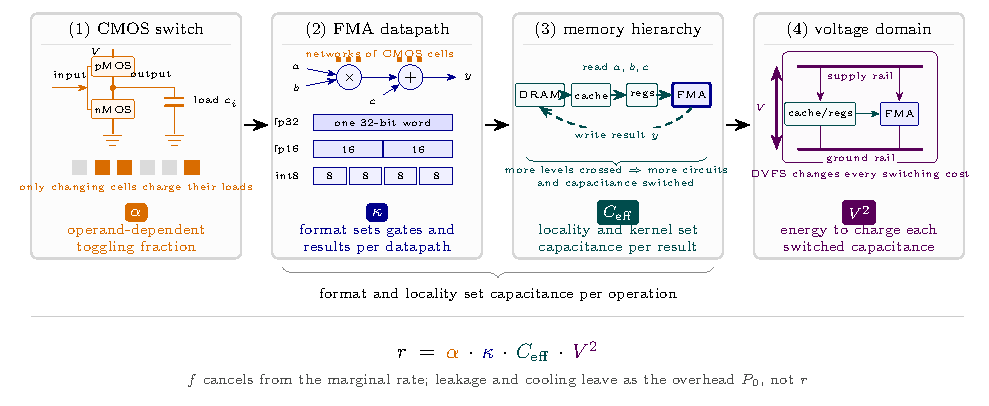
\includegraphics[width=\linewidth]{exchange_scales}
\end{minipage}\par
\postercaption{Figure 2. The exchange rate assembled across physical
scales, from a single CMOS switch to the powered die.}

% --- MEASUREMENT ----------------------------------------------------------------
\postersection{Experiments: measuring the hiding room}
\vspace{0.2cm}
\noindent
\begin{minipage}[c]{0.55\linewidth}
\bulletitem{Matmul sweep (format $\times$ operands $\times$ locality):
declared work prices anywhere from $19.5$ down to $0.786$\,pJ/op --- a
$24.8\times$ span, reproducing across four A100s to $2$--$3\%$.}
\bulletitem{Idle-state sweep: the overhead $P_0$ ranges over
$63$--$96$\,W --- joules a prover frees by idling services.}
\bulletitem{Covert dosing: covert work added to a declared burst costs
$0.51$\,pJ/op at the margin for synthetic matmuls, rising to
$2.5$--$3.2$\,pJ/op for a real transformer block (Pythia-6.9B).}
\end{minipage}\hfill
\begin{minipage}[c]{0.38\linewidth}
\centering
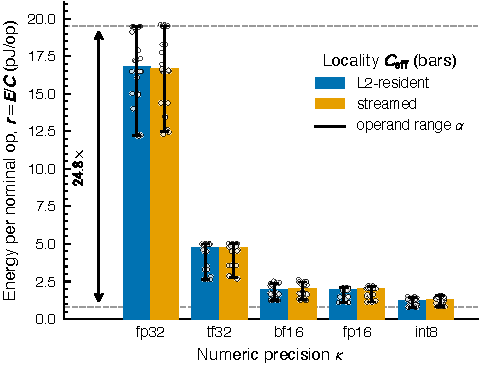
\includegraphics[width=\linewidth]{exchange_band}
\end{minipage}\par
\postercaption{Figure 3. The measured energy quotient $E/C$, swept
factorially over precision (bar groups), locality (paired bars) and
operand distribution (whiskers); dashed lines mark the band edges.}

% --- RESULTS ---------------------------------------------------------------------
\postersection{Pushing down $\beta$}
\vspace{0.2cm}
\noindent
\begin{minipage}[c]{0.59\linewidth}
\bulletitem{Power alone concedes a lot: our cheating strategies
demonstrably hide $\beta=$\textbf{0.41 machines}}
\bulletitem{Additional verifier capabilities push it down, e.g. re-executing the
declared work at an observed operating point $\beta \to \textbf{0.34}$.}
\bulletitem{Reasonable assumptions push it down further, e.g. assuming
the adversary needs \emph{useful} covert work (multiplying zero matrices
is cheap and easy to hide, but useless) $\beta \to \textbf{0.07}$}
\end{minipage}\hfill
\begin{minipage}[c]{0.35\linewidth}
\centering
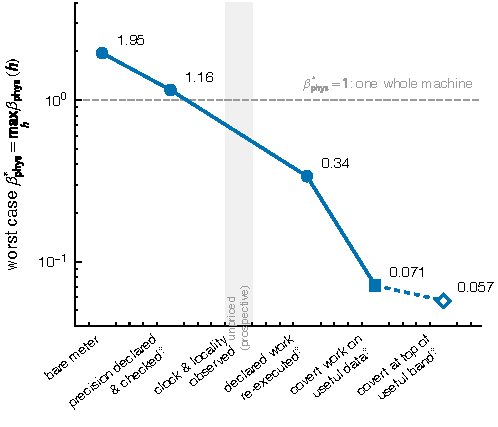
\includegraphics[width=\linewidth]{capability_ladder}
\end{minipage}\par
\postercaption{Figure 4. The capability ladder: worst-case covert compute
$\beta^{*}$ (machines of declared capacity) as the verifier gains
capabilities --- model upper bounds, whereas the 0.41 in the text is what
our cheating runs actually attained. The dashed line marks one whole
machine of conceded ambiguity.}

% --- LIMITATIONS & IMPLICATIONS ------------------------------------------------
\postersection{Limitations \& implications}
\textbf{Limitations.} One GPU model measured\redsep voltage axis
unswept\redsep power read from on-die NVML telemetry, not an off-chip
meter ($\pm5\%$ adopted)\redsep the floor prices a cheating corner, so it
is an upper bound.

\vspace{0.25cm}
\textbf{Implications.} Power traces are a viable but limited channel for
compute verification\redsep governance protocols should treat power as
one layer in a suite of verification options.

\vspace{0.25cm}
\textbf{Companion work.} Reading time resolved power, rather than the integral, the same
meter \emph{can} detect the cadence of synchronous training (WIP, repository
in sidebar).

\end{minipage}
\end{column}

\end{columns}
\end{frame}
\end{document}
